%% This file is part of the DiffractionMicroscopy project
%% Copyright 2015 David W. Hogg

% To-Do list
% ----------
% - title is a mess
% - perhaps re-phrase everything in terms of INVERSE variance?
% - possible confusions between the variance of the $k$-space Gaussian and the inverse variance of the $x$-space Gaussian!

% Style notes
% -----------

\documentclass[12pt]{article}
\usepackage{amsmath, amssymb, mathrsfs, url, graphicx}
\input{vc}

% useless formatting
\linespread{1.08333} % 10/13 spacing
\setlength{\parindent}{2\baselineskip}\addtolength{\parindent}{-1.25ex}
\setlength{\parskip}{0ex}
\newcommand{\hoggcaption}[1]{\caption{\textsf{#1}}}
\renewcommand{\thefigure}{\textsf{\arabic{figure}}}
\renewcommand{\figurename}{\textsf{Figure}}

% text definitions
\newcommand{\doi}[1]{{\footnotesize \url{http://doi.org/#1}}}

% math definitions
\newcommand{\normal}{\mathscr{N}}
\newcommand{\Poisson}{\mathscr{P}}
\newcommand{\sqnorm}[1]{|{#1}|^2}
\newcommand{\unitvec}[1]{\hat{#1}}
\newcommand{\ehat}{\unitvec{e}}
\newcommand{\xhat}{\unitvec{x}}
\newcommand{\yhat}{\unitvec{y}}
\newcommand{\zhat}{\unitvec{z}}
\newcommand{\transpose}{^{\mathsf{T}}}
\newcommand{\given}{\,|\,}
\newcommand{\setof}[1]{\left\{{#1}\right\}}
\newcommand{\dd}{\mathrm{d}}
\DeclareMathOperator{\trace}{tr}

\begin{document}\sloppy\sloppypar

\section*{\raggedright%
  Reconstruction of (the norm of) the Fourier transform
  from noisy diffraction images taken at unknown orientations: The Gaussian case}
\noindent
David W. Hogg%
\footnote{Simons Center for Data Analysis, Simons Foundation}%
\footnote{Center for Cosmology and Particle Physics, Department of Physics, New York University}%
\footnote{Center for Data Science, New York University}%
\footnote{david.hogg@nyu.edu}

\bigskip

\paragraph{Abstract:}
In certain kinds of diffraction-microscopy problems, the sample being
imaged is only in the x-ray beam for a short time, and at unknown
orientation (Euler angles), leading to a noisy image of one 2-d slice
of the squared norm of the full 3-d Fourier Transform.
In principle, many of these noisy slice images can be combined to
reconstruct the full 3-d function.
However, the fact that the orientations are unknown makes this
difficult.
Here we present a fully probabilistic approach to this problem, which
reconstructs the full 3-d function, marginalizing out the Euler
angles.
We show that, in the highly restricted case of a Gaussian molecule,
the reconstruction can be performed, even in the absurd limit in which
there is only \emph{one photon detected in each image}.
That is, the reconstructon is possible even as the information content per
image approaches zero.
There are, however, requirements on the total information content in
the data set, and on the true distribution of Euler angles.
The problem setup is artificially simple, but nothing fundamental
about the method depends on the assumption of a Gaussian molecule; in
principle this method can work for molecules of arbitrary complexity.

\section{Introducion}

DWH: This problem, apparently, is an important problem.  State it clearly
and cite some literature (see references below).

DWH: State the basic reasoning behind the approach and why,
counter-intuitively, it should work.

DWH: Point out that although this case is extremely boring and
unrealistic, there is nothing in prinicple that makes it different
from much more complex cases.

\section{Problem statement}

In a three-dimensional (3-d) space there exists a 3-d multivariate
Gaussian-shaped density blob $f(x)$.
The Fourier transform $F(k)$ in 3-d reciprocal space $k$ will
also be a Gaussian-shaped density blob.
\begin{eqnarray}
  F(k) &=& a\,\normal(k\given 0, V)
  \quad ,
\end{eqnarray}
where $a$ is some kind of amplitude and $\normal(k\given\mu, V)$ is a
Gaussian pdf for $k$ with 3-vector mean $\mu$ and $3\times 3$ variance
tensor $V$.
Without loss of generality we are going to presume a variance tensor
$V$ with principal axes aligned with the coordinate axes $\ehat_1$,
$\ehat_2$, and $\ehat_3$ directions:
\begin{eqnarray}
  V &=& \sum_{d=1}^3 \sigma^2_d \, \ehat_d\cdot\ehat_d\transpose
  \quad ,
\end{eqnarray}
where $V$ is a symmetric $3\times3$ tensor, the vectors are column
orthonormal unit vectors (so the vector products
$\ehat_d\cdot\ehat_d\transpose$ are outer products), the $\sigma^2_d$ are
scalar eigenvalues (principal variances).
Still without loss of generality we can assume that the corresponding
eigenvalues of the tensor are ordered
\begin{eqnarray}
  \sigma^2_1 \geq \sigma^2_2 \geq \sigma^2_3 > 0
  \quad .
\end{eqnarray}
Just as a reminder, the eigenvalues $\sigma^2_d$ have dimensions of
inverse length squared, since they are $k$-space variances.

We don't get to observe this Gaussian blob or its variance tensor
directly.
Instead, we get $N$ two-dimensional (2-d) images $y_n$, each of which
contains a noisy 2-d slice of the 3-d Gaussian blob, through the origin
but along an unknown slice plane.
In the small-angle limit of diffraction imaging, this slice is along a
plane perpendicular to the illumination direction $\zhat$.
In full generality, this slice is along a Ewald sphere that kisses
that perpendicular plane at the origin.
Let's start in the small-angle limit, to keep things simple.

In detail, when we take the small-angle limit, we can think of each
image $y_n$ as being an array of $M$ pixels at
2-vector coordinates $\xi_m$ in the slice plane.
Each image pixel $m$ contains a number of photons that can be thought
of as a Poisson draw with expectation set by the evaluation of the
squared norm $\sqnorm{F(k)}$ of the three-dimensional Gaussian
blob, restricted to the $\zhat$ slice, arbitrarily rotated (in 2-d).
(Actually, in detail, each pixel has expectation set by an
\emph{integral} of the squared norm of the blob, over the surface of
the pixel; we will ignore this integral for now, and just evaluate.)
None of the projection directions $\zhat_n$ or 2-d rotations are
known; only the noisy images are given.

Amusingly, in the limit in which the image is filled densely with
tiny pixels, each pixel will (with arbitrarily high probability) be
either empty or contain exactly one photon.
In this limit, each image $y_n$ can be thought of as simply a photon
list, or a set $\setof{\xi_{nk}}_{k=1}^{K_n}$ of $K_n$ photons $k$,
each with position $\xi_{nk}$.

The variance tensor of the 2-d Gaussian blob appearing in image $y_n$
is given by a slice and rotation of the 3-d inverse-variance tensor:
\begin{eqnarray}
  V_n &=& [P_n\transpose\cdot V^{-1}\cdot P_n]^{-1}
  \quad ,
\end{eqnarray}
where $P_n$ is a $3\times 2$ rectangular projection matrix, that
performs the slice and rotation.
Each rectangular projection matrix $P_n$ has three degrees of freedom or three
parameters (in some sense), which can be thought of as the Euler
angles, which are two angles on the sphere to define the direction of
$\zhat_n$ and one more angle to define the direction of the x-axis of
the image in the projection plane.

In detail, if one has the orthonormal unit 3-vectors
$\xhat_n,\yhat_n,\zhat_n$ that define the x-direction on the image
slice plane (but in the 3-d $k$-space), the y-direction on the image
slice plane, and the normal to the image slice plane, the $3\times 2$
projection matrix $P_n$ becomes
\begin{eqnarray}
  P_n &\equiv& [\xhat_n\,,\,\yhat_n]
  \quad ,
\end{eqnarray}
which (because $\xhat_n,\yhat_n$ are 3-vectors) is a $3\times2$ matrix.
This object $P_n$ might look like it has six parameters, but it is
constructed from two orthonormal vectors, so it really only has three
degrees of freedom, which correspond to the Euler angles.
Some example artificial data, made from random slices of an
anisotropic 3-d Gaussian, are shown in
\figurename~\ref{fig:exampledata8}, \ref{fig:exampledata4}, and \ref{fig:exampledata0}.
\begin{figure}[!htp]
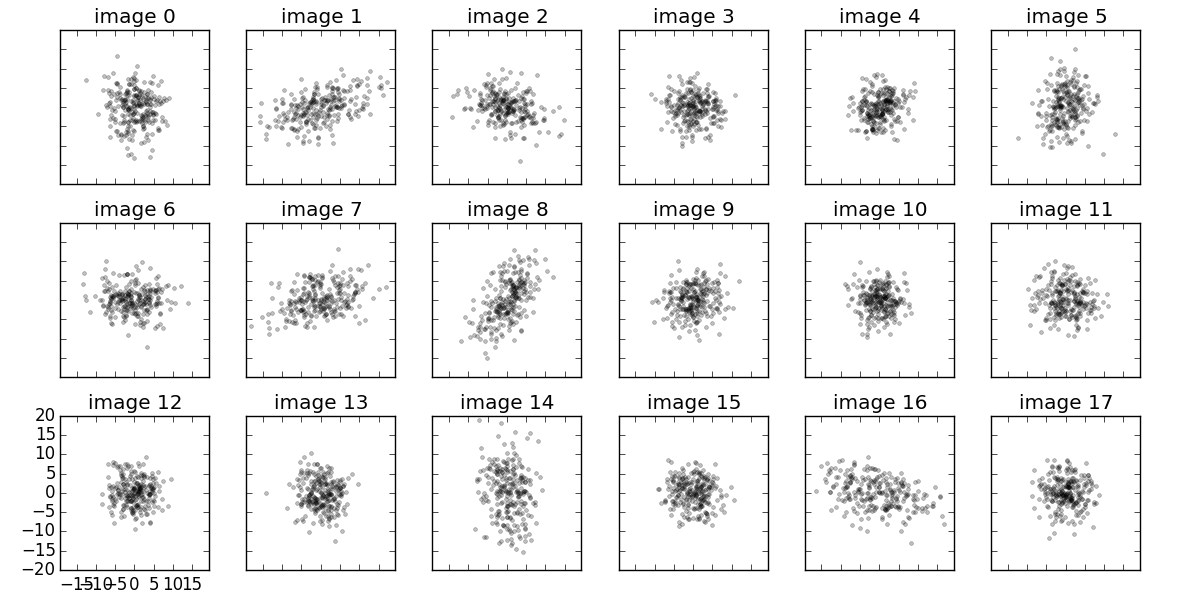
\includegraphics[width=\textwidth]{data_08_08.png}
\hoggcaption{Some example artificial data, from a data set made with
  $N=256$ images, each with $K=256$ photons, random Euler angles, and
  an anisotropic 3-d Gaussian with axis-aligned variances
  $\setof{\sigma^2_d}_{d=1}^3 = (47, 13, 11)$.\label{fig:exampledata8}}
\end{figure}
\begin{figure}[!htp]
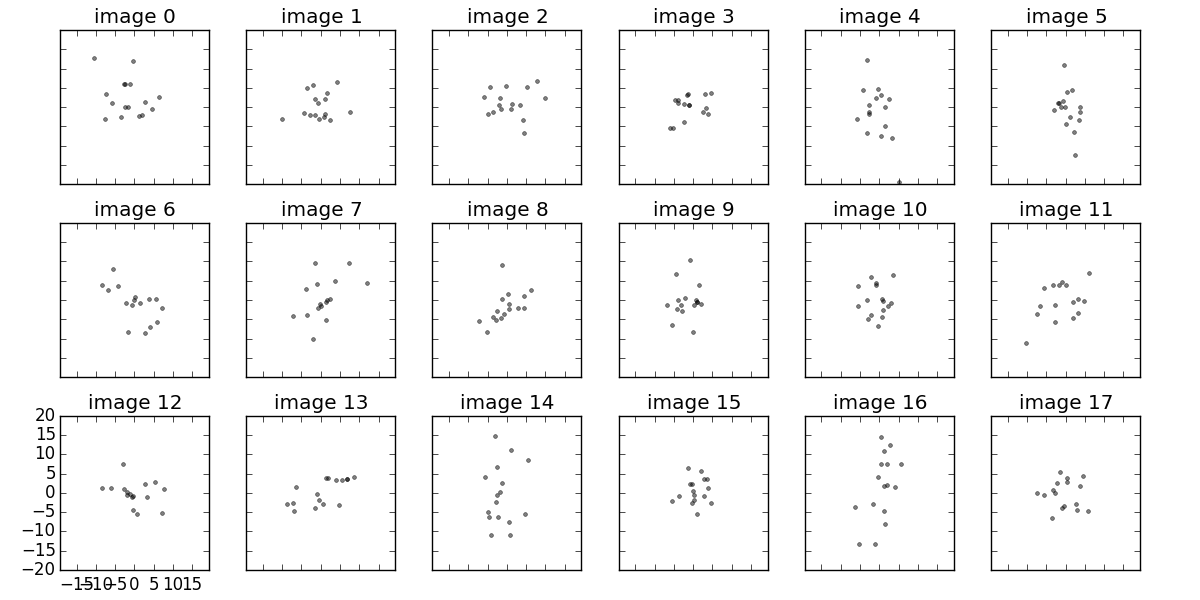
\includegraphics[width=\textwidth]{data_12_04.png}
\hoggcaption{Same as \figurename~\ref{fig:exampledata8} but from a data set made with
  $N=4096$ images, each with $K=16$ photons.\label{fig:exampledata4}}
\end{figure}
\begin{figure}[!htp]
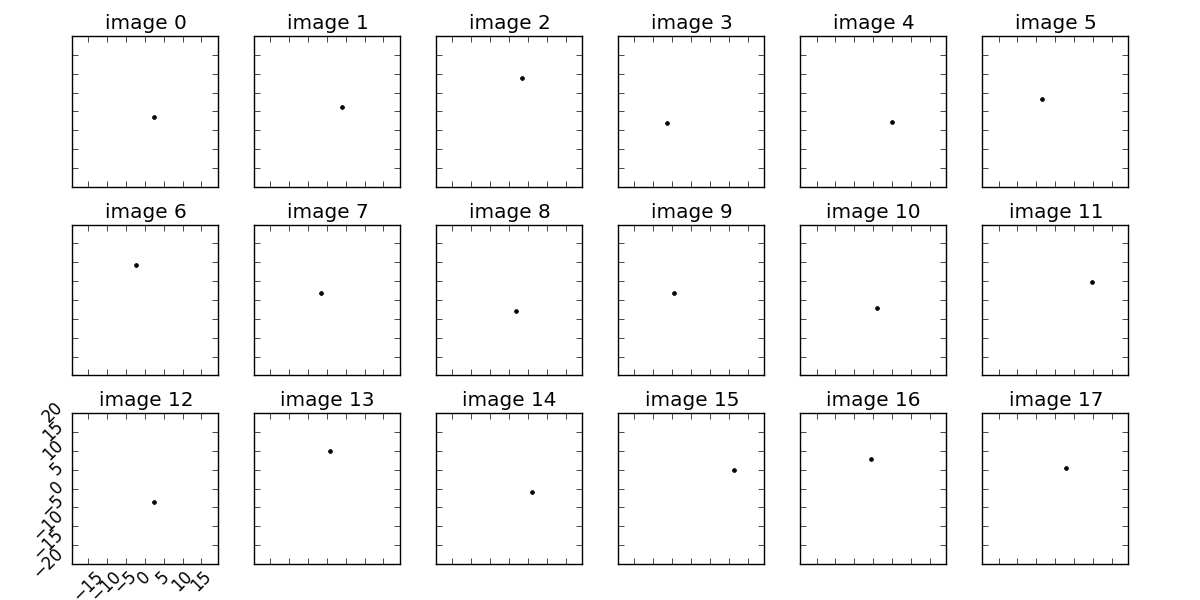
\includegraphics[width=\textwidth]{data_16_00.png}
\hoggcaption{Same as \figurename~\ref{fig:exampledata8} but from a data set made with
  $N=65536$ images, each with $K=1$ photon!\label{fig:exampledata0}}
\end{figure}

The question is:
Given these data, \emph{can we infer the 3-d variance tensor $V$?}
And if we can, how accurately, and what does it depend on?  We are
going to attempt the inference by maximizing a marginalized
likelihood, marginalizing out all $3\,N$ unknown projection and
rotation parameters.

\section{Marginalized likelihood}

Our single-pixel likelihood will be based on the Poisson process:
\begin{eqnarray}
  p(y_{nm}\given P_n,V) &=& \Poisson(y_{nm}\given\lambda_{nm})
  \\
  \lambda_{nm} &\equiv& \sqnorm{a\,\normal(\xi_m\given 0,V_n)}\,\Delta_m
  \quad,
\end{eqnarray}
where $y_{nm}$ is the $m$th pixel value in image $y_n$,
$\lambda_{nm}$ is the evaluation of the squared norm of the Fourier
transform at the pixel center (just evaluation, not integral),
$\Delta_m$ is the effective $k$-space area of the $m$th pixel,
and $\Poisson(k\given\lambda)$ is the Poisson probability for obtaining
count $k$ given expectation $\lambda$.
The likelihood is a function of the projections $P_n$ and the
three-space tensor $V$, through their combination $V_n$.

If we drop (don't infer) normalizations, and presume that all pixels
have the same effective area $\Delta_m$ in $k$-space, then this leads
to a log-likelihood
\begin{eqnarray}
  \ln p(y_n\given P_n,V) &=& \sum_{m=1}^M \ln p(y_{nm}\given P_n,V)
  \\
  \ln p(y_{nm}\given P_n,V) &=& y_{nm}\,\ln\sqnorm{\normal(\xi_m\given 0,V_n)} + \mbox{const}
  \\
  \ln p(y_{nm}\given P_n,V) &=& y_{nm}\,\ln\normal(\xi_m\given 0,\frac{1}{2}\,V_n) + \mbox{const}
  \quad,
\end{eqnarray}
where we are ignoring constants, and where we have used that the square
of a Gaussian pdf is proportional to a Gaussian pdf with half the variance.
In the dense-image-of-small-pixels limit, this can be re-written as a
sum over photons:
\begin{eqnarray}
  \ln p(y_n\given P_n,V) &=& \sum_{k=1}^{K_n} \ln p(y_{nk}\given P_n,V)
  \\
  \ln p(y_{nk}\given P_n,V) &=& \ln\normal(\xi_{nk}\given 0,\frac{1}{2}\,V_n) + \mbox{const}
  \quad.
\end{eqnarray}

Now what we really want is to marginalize out the projections and
offsets.
We are going to think of the rectangular projection matrix $P_n$ as
being controlled by a set of Euler angles $\phi$ and we are going to
marginalize these out, using an isotropic prior.
\begin{eqnarray}
  \ln p(y_n\given V) &=& \ln\int p(y_n\given P_{\phi},V)\,p(\phi)\,\dd\phi
  \quad,
\end{eqnarray}
where now we subscript $P_{\phi}$ with the Euler angles and integrate
over them.
This marginalized likelihood has the horrifying form of a log of an
integral of an exponential of a simple log-likelihood.  That's bad.

We make things little better by replacing this integral with a
sampling approximation.
If we have $T$ samples $P_t$ of rectangular projection matrices, drawn
from an isotropic distribution of Euler angles $\phi$, the
marginalized likelihood can be approximated by
\begin{eqnarray}
  \ln p(y_n\given V) &=& \ln\left[\frac{1}{T}\,\sum_{t=1}^T p(y_n\given P_t,V)\right]
  \quad,
\end{eqnarray}
where now we have a log-sum-exp form (since it is $\ln p(y_n\given
P,V)$ that has the simple form).

DWH: Expression for the derivatives?

DWH: Implementation notes and details?

DWH: How dense does the sampling have to be?  One answer is that it
has to be dense enough that the inferences don't change as the density
function is rotated in $k$-space.  For our purposes, it means we
should get the same marginalized likelihood (to a precision that is
$\ll 1$) when we re-order the principal axes of the body.  DWH: FIGURE HERE.

DWH: Also concept of effective number of samples?

\section{Experiments}

\paragraph{Performance as a function of image and photon counts:}
DWH: Hello World!

DWH: As a performance metric, we will use the symmetrized K--L
divergence $S$, which in the case of 3-d, zero-mean, multivariate
Gaussians, is:
\begin{eqnarray}
  S &\equiv& \frac{1}{2}\,\left[\trace(V_1^{-1}\cdot V_2)
                              + \trace(V_2^{-1}\cdot V_1)
                              - 6\right]
  \quad,
\end{eqnarray}
where $V_1$ and $V_2$ are the variance tensors of the two Gaussians
being compared.

\paragraph{Information content in low-photon images:}
DWH: Hello World!

DWH: Prediction: The effective number of samples gets smaller as the
number of photons per image increases.  The need for denser
$\phi$-space sampling increases as the number of photons per image
increases.

DWH: Prediction: The only $K=1$ images that have significant angle
information are images with photons at anomalously large radius or
anomalously small radius.

\paragraph{Effects of wrong orientation priors:}
DWH: Hello World!

DWH: Prediction: A wrong orientation prior will hurt more as the
number of photons per image drops.

\section{Discussion}

DWH: Hello World!

DWH: Didn't deal with censoring; how would things change if I did?

DWH: Make the Jeremy Magland argument that you could have done this
restricted case with some clever empirical statistics!  Hence: No
mystery.  The mystery is that the arguments for this approach make no
assumptions about the form or complexity of the density.

\bigskip

It is a pleasure to thank Leslie Greengard (SCDA) and Jeremy Magland
(SCDA) for valuable discussions.
This work was supported by [DWH GRANT NUMBERS].

Everything in this project, including this document itself, is
available at \giturl.  If you want this exact version, clone at git
hash \texttt{\githash~(\gitdate)}.

\section*{Possibly relevant literature}\raggedright
\begin{trivlist}
\item
Bortel, G., Faigel, G., Tegze, M., 2009,
Classification and averaging of random orientation single macromolecular diffraction patterns at atomic resolution,
J Struct Biol 166(2) 226--233.
\item
Huldt, G., Szoke, A., Hajdu, J., 2003,
Diffraction imaging of single particles and biomolecules,
J Struct Biol 144(1--2) 219--227.
\item
Martin, A. V., 2014,
The correlation of single-particle diffraction patterns as a continuous function of particle orientation,
Philos Trans R Soc Lond B Biol Sci 369(1647) 20130329
\doi{10.1098/rstb.2013.0329}.
\item
Tegze, M., Bortel, G., 2012,
Atomic structure of a single large biomolecule from diffraction patterns of random orientations,
J Struct Biol 179(1) 41--45
\doi{10.1016/j.jsb.2012.04.014}.
\end{trivlist}

\end{document}
